\documentclass[xcolor={dvipsnames}, 11pt]{beamer}
\usetheme{JuanLesPins}
%\usepackage{beamerthemeAmsterdam}

\setbeamercolor*{palette primary}{use=structure,fg=White,bg=CadetBlue!70!RoyalBlue}
\setbeamercolor*{palette quaternary}{fg=White,bg=Periwinkle}
\setbeamercolor*{item}{fg=CadetBlue}
\setbeamertemplate{navigation symbols}{}
\setbeamertemplate{caption}[numbered]

\usepackage[serbian]{babel} 
\usepackage[utf8]{inputenc} 
\usepackage{amsmath}
\usepackage{amsfonts}
\usepackage{amssymb}
\usepackage{graphicx}
\usepackage{multicol}

\author{Ajzenhamer Nikola \\ Bukurov Anja \\ Stanković Vojislav \\ Stanković Una }
\title{Neki elementi kompiliranja funkcionalnih programskih jezika}

%\logo{\includegraphics[height=1.8cm]{logo.png}\vspace{220pt}}

%institute{}

%date{}

%subject{}

%setbeamercovered{transparent}

%setbeamertemplate{navigation symbols}{}

\begin{document}
%	\maketitle

\begin{frame}
	\titlepage
\end{frame}

\section{Uvod}

\begin{frame}{Uvod}
	Funkcionalna paradigma, Džon Bakus, 1977.\\
    \tableofcontents
\end{frame}

\subsection{Osnovni pojmovi}
	
\begin{frame}{Osnovni pojmovi}
	\begin{itemize}
    \item Lambda račun
    \begin{itemize}
    \item svojstva: jednostavnost i izražajnost
    \item primena: \texttt{(f a\_1 a\_2 \ldots\ a\_n)}
    \item redukcija: \texttt{(+ 1 2)} $\rightarrow$ \texttt{3}
    \item apstrakcija: \texttt{(}$\lambda$\texttt{x.E)}
    \end{itemize}
    \item Polimorfizam
    \begin{itemize}
    \item Polimorfni programski jezici, polimorfne funkcije, polimorfni tipovi
    \item Parametarski polimorfizam
    \end{itemize}
    \end{itemize}
\end{frame}
	
\section{Elementi kompilatora}

\subsection{Efikasan kod}

\begin{frame}{Transformacije lambda računa}
	\begin{itemize}
		\item Efikasnost izvršavanja je jedan od najvažnijih problema
		\item Lambda račun se koristi zbog jednostavnosti i izražajnosti
		\item 2 grupe transformacija:
		\begin{itemize}
			\item jednostavnije (lokalne): umetanje, simplifikacija 
			\item složenije (globalne): analiza strogosti
		\end{itemize}
	\end{itemize}
\end{frame}

\begin{frame}{Umetanje}
	\begin{itemize}
		\item Dobar metod za unapređivanje performansi programa	
		\item Osnovni princip: funkcijski poziv zameniti telom funkcije
		\item Tri transformacije
		\begin{enumerate}
			\item samo umetanje (engl. inlining itself)
			\item eliminacija mrtvog koda (engl. dead code elimination)
			\item $\beta$-odsecanje (engl. $\beta$-reduction)
		\end{enumerate}
	\end{itemize}
	
	\begin{block}{Primer}
		\texttt{let \{f = $\lambda$ x.x*4\} in (f (a*b - c)) + a*d
			$\stackrel{\text{inline f}}{\longrightarrow}$ \\ let \{f = $\lambda$ x.x*4\} in (($\lambda$ x.x*4) (a*b - c)) + a*d \\ $\stackrel{\text{dead f}}{\longrightarrow}$ (($\lambda$x.x*4) (a*b - c)) + a*d \\
			$\stackrel{\beta}{\longrightarrow}$ (let {x = a*b - c} in x*4) + a*d}
	\end{block}

	
\end{frame}

\begin{frame}{Uparivanje šablona}
	\begin{itemize}
		\item Funkcije nad običnim tipovima mogu se defnisati preko različitih slučajeva
		\item Slučajevi su dati šablonima
		\item Promenljive šablona vezuju se za odgovarajuće promenljive komponente vrednosti kojoj šablon odgovara
	\end{itemize}

	\begin{block}{Primer}
		\texttt{fibonaci n
                  \\ | n==0 = 1
                  \\ | n==1 = 1
                  \\ | otherwise = (fibonaci (n-1))+(fibonaci (n-2))}
	\end{block}

\end{frame}


\subsection{Provera tipova}

\begin{frame}{Zaključivač tipova}
	
	\begin{itemize}
		\item Moderni jezici imaju svojstvo koje omogućava programeru da ne navodi tipove objekata
		\item Od velike koristi programeru jer mu ukazuje na greške
		\item Pri izvršavanju se neće javiti greške poput upotrebe promenljive tipa \texttt{bool} kao da je tipa \texttt{int}
		\item Proces zaključivanja tipova
		\begin{itemize}
			\item uparivanje tipova operatora
			\item instanciranje tipova promenljivih
		\end{itemize}
	\end{itemize}
	
\end{frame}


\subsection{Sakupljači otpadaka}
\begin{frame}{Motivacija}
	\begin{itemize}
		\item Otpaci su delovi memorije koji nisu dostupni za alociranje
		\item Sakupljač otpadaka eliminiše otpatke
		\item Ukoliko se otpatci ne eliminišu dolazi do curenja memorije
		\item Sakupljač otpadaka je potreban funkcionalnim programskim jezicima
	\end{itemize}
\end{frame}

\begin{frame}{Tipovi sakupljača otpadaka}
	\begin{itemize}
		\item Markirajući sakupljač otpadaka
		\item Sakupljač otpadaka sa brojanjem referenci
		\item Prepisujući sakupljač otpadaka
		\item Generacijski sakupljač otpadaka
	\end{itemize}
\end{frame}



\section{Apstraktne mašine}
\subsection{Uvod}
\begin{frame}{Motivacija}
	\begin{figure}[H]
 		\centering
 		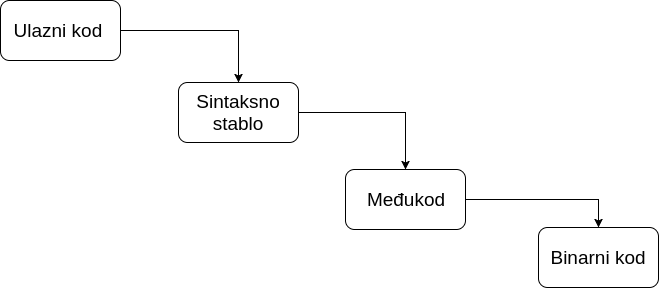
\includegraphics[width=\textwidth,height=\textheight,keepaspectratio]{slika1.png}
 		\caption{Vizuelni prikaz prevođenja k\^ oda.}
 		\label{fig:primerGmasine}
 	\end{figure}
\end{frame}

\begin{frame}{Vrste apstraktnih mašina}

	\begin{itemize}
	\item SECD mašina
	\item STG mašina
	\item G mašina
	\end{itemize}

\end{frame}

\subsection{SECD mašina}

\begin{frame}{SECD mašina}
	\begin{itemize}
	\item Jedna od prvih mašina za izvršavanje funkcionalnih programskih jezika
	\item Osnovna uloga je izvršavanje kompiliranog koda
	\item Formalno, SECD mašina je torka četiri liste sa precizno definisanim skupom operacija nad njima
	\item Komponente torke su četiri steka: 
		\begin{itemize}
		\item S (engl. stack)
		\item E (engl. environment)
		\item C (engl. control)
		\item D	(engl. dump)
		\end{itemize}
	\end{itemize}
	
\end{frame}

\subsection{G-mašina}
\begin{frame}{G mašina}
	\begin{itemize}
		\item Osnovna uloga G mašine je redukovanje grafa izračunavanja
		\item Osnovna ideja je da: 
			\begin{itemize}
			\item program predstavimo grafom
			\item evaluacijom deljenog podgrafa automatski razrešimo sve izraze koji pokazuju na njega
			\item graf $"$prepišemo$"$ evaluacijom
			\end{itemize}
		\item Važni koncepti:
			\begin{itemize}
			\item ne postoje promenljive, već imenovani izrazi
			\item vrednosti funkcije ne zavise ni od čega, osim od argumenata funkcije
			\end{itemize}				
	\end{itemize}
\end{frame}

% TODO: Srediti da se ova slika lepo prikazuje
% Sređeno :D
% <3!

\section{Zaključak}
\begin{frame}{Zaključak}
	\begin{itemize}
		\item Fokusirali smo se na određeni podskup tehnika i procesa koji omogućavaju efikasno
		kompiliranje koda
		\item Lambda račun kao međujezik za kompiliranje funkcionalnih programskih jezika
		\item Efikasan izvršni k\^ od je veoma važan za sve programske jezike
		\item Polimorfna provera tipova je korisno svojstvo programskih jezika koje veoma olakšava posao programerima
		\item Programiranje u funkcionalnim programskim jezicima se ne može zamisliti bez podrške koju pružaju sakupljači otpadaka 
		\item Apstraktne mašine predstavljaju prelaz između jezika visokog nivoa i arhitekture niskog nivoa
	\end{itemize}
\end{frame}


\section{Literatura}
\begin{frame}{Literatura}
	
	\begin{thebibliography}{10}
		
		\beamertemplatearticlebibitems
		\bibitem{}
			Simon L. Peyton Jones
			\newblock The Implementation of Functional Programming Languages	
			\newblock Prentice Hall 1987.
		
		\beamertemplatearticlebibitems
		\bibitem{}
			R. Wilhelm and H. Seidl
			\newblock Compiler Design
			\newblock Springer 2010.
		
		\beamertemplatearticlebibitems
		\bibitem{}
			Robert W. Sebesta 
			\newblock Concepts of programming languages, 10th ed.
			\newblock Pearson 2009.
			
	\end{thebibliography}
\end{frame}

\section{}
\begin{frame}
	\centering \Large Hvala na pažnji!
\end{frame}
	
	
\end{document}
